\documentclass{article}
\usepackage{amsmath}
\usepackage{graphicx}

\begin{document}

\title{Monte Carlo, Markov Chains, and Monopoly}
\author{Evan Henke}

\maketitle

\begin{abstract}
This is abstract text: This simple document shows very basic features of
\LaTeX{}.
\end{abstract}


\section{Introduction}

Whether you enjoy the game or not, everyone in their lifetime has played a game of \textit{Monopoly}.  It has been around for over 70 years and in that time has become one of the world’s most played and most well known board games.  The game pits a few friends against each other to see who can make the most money.  Every player has a pawn that they will move around the board, the distance each pawn moves depends on the outcome of a roll of two dice.  Naturally, this causes the game to rely heavily on randomness because a player can choose if they want to purchase a property, but they cannot directly choose which property they are going to buy.  Much of the game can be boiled down to only one, true question each player needs to answer: "Should I buy the property I just landed on?"  That is the goal, when a player lands on a property, should they buy it?  More mathematically speaking, at what probability should the player purchase a property, knowing which side of the board they are on.

\subsection{History and Gameplay}

People have been playing \textit{Monopoly}, or games similar to it, for close to a century.  But most people are unaware that \textit{Monopoly} is a derivative of a different board game called \textit{The Landlord’s Game}.  Originally created by a woman named Elizabeth Magie, \textit{The Landlord’s Game} was made as an education tool.  Magie was a Georgist, meaning she believed in the philosophies of Henry George whose pinnacle belief was that any economic value that is derived from land should be divided equally among all members of society.  She believed this could be difficult to teach or explain, therefore she decided to create a board game to demonstrate the process of land grabbing, the practice of large-scale purchase of land for economic profit.

\textit{Monopoly} is not advertised as a sinister game, it is portrayed as vibrantly-colored, fun, family game where to goal just happens to be to have the most money at the end of the game.  But it becomes obvious while playing that aquiring the most money will come at the expense of everyone else who is playing.  That is what Magie meant to show, but more specifically that rent strengthens the landlord at the expense of the tenant.


\begin{figure}
    \centering
    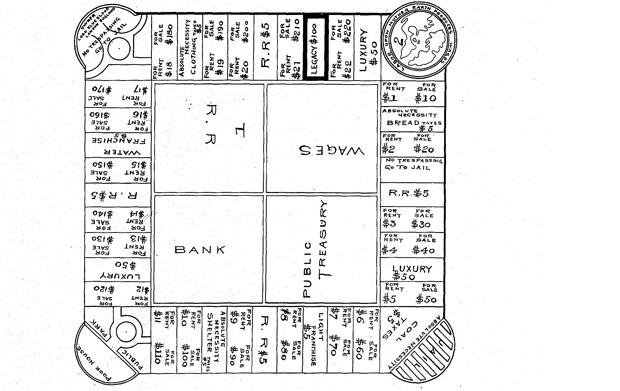
\includegraphics[width=4.0in]{landlordsgame}
    \caption{Early rendition of \textit{The Landlord's Game}}
    \label{landlordsgame_image}
\end{figure}


Magie had her game patented in 1904 and she approached Parker Brothers to produce it.  Parker Brothers refused due to the games complexity but she was determined and she was able to have her game produced by smaller publishing companies and over time the game spread. But, with popularity comes imitation, and soon enough many others would try to replicate The Landlord’s Game and its success.  The most notably being \textit{Monopoly}, which ironically, was produced by Parker Brothers and claimed to have been created solely by a man named Charles Darrow.

Parker Brothers began production of \textit{Monopoly} in 1935, this is when it began to take the form that most people recognize, with the iconic mascot Rich Uncle Pennybags following a few years later.  The board has nine spaces on each side with one space on each corner: Go, Jail, Go to Jail, and Free Parking, for a total of 40 spaces.  Each space on the board is different, there are five properties available for player purchase on the first and four side and six on the second and third side.  There are two sets of color coded properties on each side of the board and if one player owns both or all three properties in the set, then they are said to have a monopoly at that location on the board.  There is also one utility property on each side of the board as well as three Chance spaces, three Community Chest spaces, and two Tax spaces scattered around the board.  Also in the box are 32 house pieces and 12 hotel pieces.

Every player will begin the game with 1200 dollars and their pawn will start on Go and, on their turn, the player will roll two dice and move the number of spaces indicated by the sum of their roll.  Depending on where the player lands due to their dice roll, they would have to take a certain action.  Chance and Community Chest spaces make the player draw a card and take an action depending on the card text, whereas the Tax spaces requires the player to simply lose the amount of money indicated on the space on the board.  If the player lands on a property then one of two things will happen depending on whether or not the property is owned.  If no one owns the property, whatever player landed on it has the opportunity to purchase it.  If they decide they want the property, they pay the indicated price on board and add that property to their collection, but if they decide not to buy it then the property is put up for auction and any player that would want to purchase that property can put a bid down for it.  Whoever is willing to pay the most will purchase the property.  If the player lands on a property that is owned by another player, they must pay a sum of money to the owner of the property that depends on whether or not the owner has a monopoly at that location.  In the event that the owned location is part of a monopoly, the amount of money owed will still vary depending on whether the monopoly has houses or a hotel.

When a player owns a monopoly, he or she has the option to purchase houses on those properties.  Each individual property will specify how much a house will cost and the player must be able to afford to put a house on every property in that monopoly if they opt to purchase houses.  For example, if a player owns a monopoly with three properties: property A requires 100 dollars for a house, property B requires 110 dollars, and property C requires 120 dollars.  The player must be able to pay the total of 330 dollars to be able to place a house on each property in that monopoly.  The amount of money the owner gains from an opposing player landing on the space increases for every house placed on that property up to a maximum of four houses.  If a player has four houses on each property in their monopoly, he or she can choose to purchase a hotel to be placed on each property.  Hotels function very similarly to houses in that the player must be able to afford to buy enough hotels as to have one on each property and they will increase the amount the owner gains if an opposing player lands there. But when a hotel is purchased, the four houses are removed from the property and will go back into the house pool.  This differentiation is important and it will be touched on in the Common Strategies portion.

There a few other important spaces on the board.  On each side there will be one of four utility tiles, these spaces function almost identically to that of normal monopoly properties in that a player earns more if they own more of those spaces, with the exception that these spaces cannot have houses or hotels.  Go is where players start and whenever a player lands on Go or passes Go they are given 200 dollars, unless stated otherwise by a card action.  Free parking is a free space and nothing happens when a player ends their turn at that location.  The Go to Jail sends the player to Jail if they end their turn there.  Jail is the final special space that needs mentioning because it is fairly important.  Jail is the second corner that a player will pass when rounding the board and it is two spaces in one: In Jail or Just Visiting.  If the player is moving by normal means onto the jail space they are said to be just visiting and nothing special happens, it is similar to free parking in that way. But if the player lands on the Go to Jail space or are sent to jail by a card action, then their pawn is moved to the Jail space and they are said to be in jail.  If a player is in jail they can do one of two things, roll the dice or pay 50 dollars.  Paying 50 dollars will place them into the Just Visiting part of the space and they can continue to play on their next turn.  Or the player can roll the dice and if they roll doubles then they leave jail as if they had paid the 50 dollars.  If they fail the roll then they stay in jail and can retry the roll or pay the 50 dollars on their following turn.  A player can leave jail after their third turn of being in jail.
	
If a player lands and an owned property and does not have the funds to pay the owner, they can mortgage their properties.  This means they gain a small sum of money determined by the property that was mortgaged.  A mortgaged property is still owned by the same player, but the owner cannot gain income from that property though; in other words, if a player lands on a mortgaged property, they are not required to pay the owner.

A large portion of the game that is not governed by the rule book is player trading.  On a player’s turn, they can propose a trade with another player for properties or cash.  There are no true stipulations to how this trade is conducted and no player is required to accept an offer.  This gives each game of Monopoly more variety but is extremely difficult to model due to the individuality of players.

\section{The Simulation}

There are a number of things that complicate simulating \textit{Monopoly} that does not directly affect the game’s main function, which is to roll dice to move around the board and to purchase properties.  Therefore houses, hotels, Community Chest cards, Chance cards, property auctions, mortgaging, and trading have been removed to give a more bare-bones approach.

\subsection{Monte Carlo Methods}

One will notice that there are many conditionals within the rules, which can cause difficulties with the modeling approach, and this is why Monte Carlo simulations will be beneficial.  Our goal is to find some optimal probability to purchase a property on the board, but this is problematic because it depends on a very large number of factors, including each individual player’s probability to buy as well as which states are available, how much money the current player has, etc.  In \textit{Monopoly}, these previously mentioned variables rely, directly or indirectly, upon the probability of being at a specific spot on the board at a certain time.  A textbook optimization problem, in most instances, could be solved using some arithmetical approximation akin to Newton's Method.  But in this case a distinct function, \mathit{f} is not apparent, let alone finding it's derivative.

Monte Carlo simulations stress that a mathematical model can be solved using random numbers, which lends itself perfectly to this predicament.  Implementing the idea that the use of random numbers can lead to a non-random solution, we can begin to simulate games of Monopoly with random purchasing probabilities in the hopes to find optimal purchase strategies.

\subsection{Markov Chains and Finite-State Machines}

So far this is an extremely general starting point, it has been established that there are going to be a huge number of games played, now what?  Following the rules in playing order says that the first thing a player is going to do is to roll two dice to move their pawn around the board, so there needs to be a way to move their pawn.

\subsection{Bringing It All Together}

The simulation is broken into two parts, single games and rounds.  A game, as the name implies, is only one game with a single winner.  Whereas a round constitutes playing one thousand games.  Every player will have a counter that will increase with how many games they have won per round.

Each game will start with four players, simply named Player One, Player Two, Player Three, and Player Four.  Player One is the player we will be optimizing around.  Each player will start on Go with 1200 dollars and an initial probability to buy that is randomly chosen between zero and one for each side of the board, with the exception that Player One will have a static initial probability to buy on each side of .50.  The players will cycle around the board using the transition matrix p, given by the figure later in this paper somewhere not sure where yet, the first and fourth sides of the board have five available properties to purchase and the second and third sides have six properties to purchase.  The simulation contains two arrays, one that tells if the space is available for purchase and the other array stores the owner of the property if it is owned.  When a player lands on a property the game will check both of these arrays for an owner, if the property has no owner then the player will buy the property with that player’s respective probability to buy on that side of the board.  If the property is owned the player will pay the owner an amount according to the side of the board as well as how many properties the owner has in their possession.  Each player will have a turn and if they land on a property that they cannot afford, they are removed from the game and their owned properties are returned to their unowned state and are available for purchase by the remaining players.  This will go on until one player wins.  

Once a round is complete whichever player has the most wins is deemed the round winner.  At this point the winner’s probability to win will be saved and the probabilities of Player One will be be adjusted according to the following weighted adjustment:

\begin{equation}
    \label{probability_adjustment}
    P_{i+1} = \alpha_i P_i + (1+\alpha_i)P_{winner}
\end{equation}

Where $\alpha_i$ is a constant that will be varied when the simulation is ran multiple times.

\begin{center}
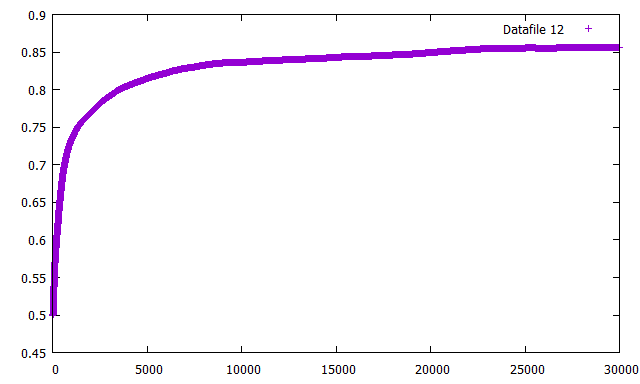
\includegraphics[width = \textwidth]{average}
\end{center}

\section{Conclusion}

Lorem ipsum dolor sit amet, consectetur adipisicing elit, sed do eiusmod tempor
incididunt ut labore et dolore magna aliqua. Ut enim ad minim veniam, quis
nostrud exercitation ullamco laboris nisi ut aliquip ex ea commodo consequat.
Duis aute irure dolor in reprehenderit in voluptate velit esse cillum dolore eu
fugiat nulla pariatur.


\end{document}